\documentclass[aps,superscriptaddress,groupedaddress]{revtex4}  % for double-spaced preprint

\usepackage{graphicx}  % needed for figures
\usepackage{float}
\usepackage{dcolumn}   % needed for some tables
\usepackage{bm}        % for math
\usepackage{amssymb}   % for math
\usepackage{slashed}   % for Dirac Slash
\usepackage{amsmath}   % for mutiline eqn
\usepackage{simplewick} % for contraction
\usepackage{verbatim}  % for multi-line comment
\usepackage{color} % for textcolor
\usepackage{appendix} % for appendix
\usepackage{epstopdf}
\usepackage{subfig}
\usepackage{listings}
\usepackage{xcolor}

% \usepackage[numbers,sort&compress]{natbib} %for cite

% avoids incorrect hyphenation, added Nov/08 by SSR
\hyphenation{ALPGEN}
\hyphenation{EVTGEN}
\hyphenation{PYTHIA}

% for bookmarks
\usepackage[bookmarks=true,colorlinks=true,linkcolor=blue,unicode=true]{hyperref}

\begin{document}

\widetext

\title{A GPU simulation of skyrmion}

\date{\today}


\begin{abstract}
A GPU simulation of skyrmion.
\end{abstract}

\maketitle

\section{\label{sec:1}LLG}

The Landau-Lifshitz-Gilbert-Equation~(LLG) can be written as (Eq.~(13) of Ref.~\cite{review1} and Eq.~(7) of Ref.~\cite{hamiton}, NOTE that the sign of the last term is `+' in Eq.~(7) of Ref.~\cite{hamiton})
\begin{equation}
\begin{split}
&\dot {\bf n}=\gamma {\bf B}_{\rm eff}\times {\bf n}-\frac{\alpha \gamma}{|n|} {\bf n}\times \dot{\bf n}-\frac{\hbar \gamma}{2e}\left({\bf j}\cdot {\bf \nabla}\right){\bf n}
\end{split}
\end{equation}
where ${\bf n}$ is the magnetic momentum, $\gamma(\gamma > 0)$ is the gyromagnetic ratio, $\alpha$ represents Gilbert damping, ${\bf B}_{\rm eff}$ is the effective field arising from the spin Hamiltonian, and can be written as ($H_S$ is from Ref.~\cite{hamiton}, before Eq.~(1), also Eq.~(4) in Ref.~\cite{pin2})
\begin{equation}
\begin{split}
&{\bf B}_{\rm eff}\equiv \frac{\delta H_S}{\delta {\bf n}}\\
&H_S=\int d^D x\frac{J}{2a} (\nabla  {\bf n})^2+\frac{D}{a^2}{\bf n}\cdot \left(\nabla \times {\bf n}\right)-\frac{\mu}{a^3}{\bf B}\cdot {\bf n}\\
\end{split}
\end{equation}

\section{\label{sec:2}LLG in 2D lattice}

In the following, for simplicity, we use $\delta = a({\bf e}_x, {\bf e}_y)$, $\delta _x=a{\bf e}_x, \delta _y=a{\bf e}_y$, where $a$ is the distance between two lattice.

\subsection{\label{sec:2.1}Spin torque}
Written in lattice, so that
\begin{equation}
\begin{split}
&\left({\bf j}\cdot \nabla\right) {\bf n}=\sum _i j_i\partial _i n_x{\bf e}_x+\sum _i j_i\partial _i n_y{\bf e}_y+\sum _i j_i\partial _i n_z{\bf e}_z\\
\end{split}
\end{equation}
In 2D, it is
\begin{equation}
\begin{split}
&\left({\bf j}\cdot \nabla\right) {\bf n}= \sum _{i=x,y}j_i(\partial _i n_x{\bf e}_x+ \partial _i n_y{\bf e}_y+\partial _i n_z{\bf e}_z)\\
&=\frac{1}{a}\sum _{i=x,y}j_i(\frac{n_{x}({\bf r}+\delta _i)-n_{x}({\bf r}-\delta _i)}{2}{\bf e}_x+ \frac{n_{y}({\bf r}+\delta _i)-n_{y}({\bf r}-\delta _i)}{2}{\bf e}_y+\frac{n_{z}({\bf r}+\delta _i)-n_{z}({\bf r}-\delta _i)}{2}{\bf e}_z)\\
&=\frac{1}{a}\sum _{i=x,y}j_i\frac{{\bf n}({\bf r}+\delta _i)-{\bf n}({\bf r}-\delta _i)}{2}
\end{split}
\end{equation}
Sometimes, it is also written as (see last term in Eq.~(8) in Ref.~\cite{pin}, it also says this is the discrete version of the continuous term $({\bf j}\cdot \nabla ){\bf n}$ before Eq.~(10))
\begin{equation}
\begin{split}
&\left({\bf j}\cdot \nabla\right) {\bf n}=\frac{1}{a}\sum _{i=x,y}j_i{\bf n}({\bf r})\times \left(\frac{{\bf n}({\bf r}+\delta _i)-{\bf n}({\bf r}-\delta _i)}{2}\times {\bf n}({\bf r})\right)
\end{split}
\end{equation}
that is because, for a unit vector, one have
\begin{equation}
\begin{split}
&{\bf n}\cdot \partial _i {\bf n}=0
\end{split}
\end{equation}
the discrete version is
\begin{equation}
\begin{split}
&{\bf n}(\bf {r})\cdot \frac{{\bf n}({\bf r}+\delta _i)-{\bf n}({\bf r}-\delta _i)}{2a}=0
\end{split}
\end{equation}
so that
\begin{equation}
\begin{split}
&{\bf n}({\bf r})\times \left(\frac{{\bf n}({\bf r}+\delta _i)-{\bf n}({\bf r}-\delta _i)}{2}\times {\bf n}({\bf r})\right)\\
&=\frac{{\bf n}({\bf r}+\delta _i)-{\bf n}({\bf r}-\delta _i)}{2}({\bf n}({\bf r})\cdot {\bf n}({\bf r}))-{\bf n}({\bf r}) \left({\bf n}({\bf r})\cdot \frac{{\bf n}({\bf r}+\delta _i)-{\bf n}({\bf r}-\delta _i)}{2}\right)\\
&=\frac{{\bf n}({\bf r}+\delta _i)-{\bf n}({\bf r}-\delta _i)}{2}\\
\end{split}
\end{equation}
to be consist with the references, we use
\begin{equation}
\begin{split}
&\left({\bf j}\cdot \nabla\right) {\bf n}=\frac{1}{a}\sum _{i=x,y}j_i{\bf n}({\bf r})\times \left(\frac{{\bf n}({\bf r}+\delta _i)-{\bf n}({\bf r}-\delta _i)}{2}\times {\bf n}({\bf r})\right)
\end{split}
\end{equation}

In simulation, to simplify, we always take the direction of ${\bf j}$ as ${\bf x}$-axis, so we only have
\begin{equation}
\begin{split}
&\frac{1}{a}j_x{\bf n}({\bf r})\times \left(\frac{{\bf n}({\bf r}+\delta _x)-{\bf n}({\bf r}-\delta _x)}{2}\times {\bf n}({\bf r})\right)
\end{split}
\end{equation}

\subsection{\label{sec:2.2}J term}

$(\nabla  {\bf n})^2$ is confusing, in 2D, it is in fact $\sum _{i=x,y}(\partial _i {\bf n})\cdot (\partial _i {\bf n})$
Consider in 1-dimension, we have
\begin{equation}
\begin{split}
&{\bf n}(x)\cdot \partial _i {\bf n}(x)=0\\
&0=\sum _{i=x,y} \partial _i\left({\bf n}(x)\cdot \partial _i {\bf n}(x)\right)=\sum _{i=x,y}(\partial _i {\bf n})\cdot (\partial _i {\bf n}) + {\bf n}\cdot (\sum _{i=x,y}(\partial _i)^2){\bf n}\\
\end{split}
\end{equation}
In lattice, the derivate can be written as
\begin{equation}
\begin{split}
&\frac{d^2}{dx^2}{\bf n}({\bf r})=\frac{1}{a}\left({\bf n}'({\bf r}+\frac{a}{2}{\bf e}_x)-{\bf n}'({\bf r}-\frac{a}{2}{\bf e}_x)\right)
\end{split}
\end{equation}
with
\begin{equation}
\begin{split}
&{\bf n}'({\bf r}+\frac{a}{2}{\bf e}_x)=\frac{1}{a}\left({\bf n}({\bf r}+a{\bf e}_x)-{\bf n}({\bf r})\right)\\
&{\bf n}'({\bf r}-\frac{a}{2}{\bf e}_x)=\frac{1}{a}\left({\bf n}({\bf r})-{\bf n}({\bf r}-a{\bf e}_x)\right)\\
\end{split}
\end{equation}
so that
\begin{equation}
\begin{split}
&(\sum _{i=x,y}(\partial _i)^2){\bf n}=\frac{1}{a^2}\sum _{i=x,y,-x,-y}{\bf n}({\bf r}+\delta _i)-4{\bf n}({\bf r})
\end{split}
\end{equation}
and
\begin{equation}
\begin{split}
&{\bf n}\cdot (\sum _{i=x,y}(\partial _i)^2){\bf n}=\frac{1}{a^2}\sum _{\langle i\rangle}{\bf n}\cdot {\bf n}_i-4
\end{split}
\end{equation}

Throw away the constant term
\begin{equation}
\begin{split}
&\int d^D x\frac{J}{2a}(\nabla {\bf n})^2=-\frac{J}{2a^3}\sum _{\langle i, j\rangle}{\bf n}_i\cdot {\bf n}_j
\end{split}
\end{equation}
where $j$ are all neighbours of $i$, $j=i+\delta_x,i-\delta_x,i+\delta_y,i-\delta_y$.

When $J$ is constant, it can also been written as
\begin{equation}
\begin{split}
&\int d^D x\frac{J}{2a}(\nabla {\bf n})^2=-\frac{J}{a^3}\sum _{{\bf r}}{\bf n}({\bf r})\cdot \left( {\bf n}({\bf r}+\delta _x)+{\bf n}({\bf r}+\delta _y)\right)
\end{split}
\end{equation}


\subsection{\label{sec:2.3}D term}

In 2D, we find
\begin{equation}
\begin{split}
&{\bf n}\cdot (\nabla \times {\bf n})=n_x \partial _y n_z-n_y \partial _x n_z+n_z\partial _x n_y-n_z \partial _y n_x\\
&=\frac{1}{2a}\left[\left(n_x({\bf r})(n_z({\bf r}+\delta _y)-n_z({\bf r}-\delta _y))-n_z({\bf r})(n_x({\bf r}+\delta _y)-n_x({\bf r}-\delta _y))\right)\right.\\
&\left.+\left(n_z({\bf r})(n_y({\bf r}+\delta _x)-n_y({\bf r}-\delta _x))-n_y({\bf r})(n_z({\bf r}+\delta _x)-n_z({\bf r}-\delta _x))\right)\right]\\
&=\frac{1}{2a}\left[\left(n_x({\bf r})n_z({\bf r}+\delta _y)-n_z({\bf r})n_x({\bf r}+\delta _y)\right)-\left(n_x({\bf r})n_z({\bf r}-\delta _y)-n_z({\bf r})n_x({\bf r}-\delta _y)\right)\right.\\
&\left.+\left(n_z({\bf r})n_y({\bf r}+\delta _x)-n_y({\bf r})n_z({\bf r}+\delta _x)\right)-\left(n_z({\bf r})n_y({\bf r}-\delta _x)-n_y({\bf r})n_z({\bf r}-\delta _x)\right)\right]\\
&=-\frac{1}{2a}\left[{\bf n}({\bf r})\cdot \left({\bf n}({\bf r}+\delta _y)\times {\bf e}_y\right)-{\bf n}({\bf r})\cdot \left({\bf n}({\bf r}-\delta _y)\times {\bf e}_y\right)\right.\\
&\left.+{\bf n}({\bf r})\cdot \left({\bf n}({\bf r}+\delta _x)\times {\bf e}_x\right)-{\bf n}({\bf r})\cdot \left({\bf n}({\bf r}-\delta _x)\times {\bf e}_x\right)\right]\\
&=-\frac{1}{2a^2}\left[{\bf n}({\bf r})\times {\bf n}({\bf r}+\delta _y)\cdot \delta_y-{\bf n}({\bf r})\times {\bf n}({\bf r}-\delta _y)\cdot \delta_y\right.\\
&\left.+{\bf n}({\bf r})\times{\bf n}({\bf r}+\delta _x)\cdot \delta_x-{\bf n}({\bf r})\times {\bf n}({\bf r}-\delta _x)\cdot \delta_x\right]\\
\end{split}
\end{equation}
so, one have
\begin{equation}
\begin{split}
&\int d^D x\frac{D}{a^2}{\bf n}\cdot (\nabla \times {\bf n})=-\frac{D}{a^4}\sum _{{\bf r}}\left({\bf n}({\bf r})\times  {\bf n}({\bf r}+\delta _x) \cdot \delta _x+{\bf n}({\bf r})\times  {\bf n}({\bf r}+\delta _y) \cdot \delta _y\right)
\end{split}
\end{equation}

It is also
\begin{equation}
\begin{split}
&\int d^D x\frac{D}{a^2}{\bf n}\cdot (\nabla \times {\bf n})=-\frac{D}{a^4}\sum _{{\bf r}}\left({\bf n}({\bf r}+\delta _x)\times \delta _x+{\bf n}({\bf r}+\delta _y)\times \delta _y\right)\cdot {\bf n}({\bf r})
\end{split}
\end{equation}

\subsection{\label{sec:2.4}Effective magnetic field}

Using the results, we can write the discrete version of $H_s$ as
\begin{equation}
\begin{split}
&H_S=\sum _{{\bf r}}\left[-\frac{J}{a^3} ({\bf n}({\bf r}+\delta_x)+{\bf n}({\bf r}+\delta_y))-\frac{D}{a^3}  ({\bf n}({\bf r}+\delta_x)\times {{\bf e}}_x+{\bf n}({\bf r}+\delta_y)\times {{\bf e}}_y)-\frac{\mu}{a^3}{\bf B}\right]\cdot {\bf n}({\bf r})
\end{split}
\end{equation}
which leads to
\begin{equation}
\begin{split}
&{\bf B}_{\rm eff}({\bf r})=\frac{\delta H_S}{\delta {\bf n}}=-\frac{1}{a^3} \sum _{i=x,y}\left[J({\bf r}){\bf n}({\bf r}+\delta_i)+J({\bf r}-\delta_i){\bf n}({\bf r}-\delta_i)\right]\\
&-\frac{1}{a^3}  \sum _{i=x,y}\left[D({\bf r}){\bf n}({\bf r}+\delta_i)\times {{\bf e}}_i-D({\bf r}-\delta _i){\bf n}({\bf r}-\delta_i)\times {{\bf e}}_i\right]-\frac{\mu}{a^3}{\bf B}({\bf r})
\end{split}
\end{equation}

\subsection{\label{sec:2.5}anisotropy}

In some material, the effective Hamiltonian can be written with anisotropy terms as (if ignore $a$, this is as same as Eq.~(10) in Ref.~\cite{spintransfer})
\begin{equation}
\begin{split}
&H_S=\sum _{{\bf r}}\left[-\frac{J}{a^3} ({\bf n}({\bf r}+\delta_x)+{\bf n}({\bf r}+\delta_y))-\frac{D}{a^3}  ({\bf n}({\bf r}+\delta_x)\times {{\bf e}}_x+{\bf n}({\bf r}+\delta_y)\times {{\bf e}}_y)-\frac{\mu}{a^3}{\bf B}\right.\\
&\left.-{\bf h}\right]\cdot {\bf n}({\bf r})-K\left({\bf e}_z\cdot {\bf n}({\bf r})\right)^2
\end{split}
\end{equation}

The contribution of ${\bf h}$ can be just put into the applied magnetic field ${\bf B}$, we also include the contribution of $K$.

\subsection{\label{sec:2.6}dimensionless LLG}

Using $\tau = \gamma t$
\begin{equation}
\begin{split}
&\frac{d}{d\tau} {\bf n}= {\bf B}_{\rm eff}\times {\bf n}-\frac{\alpha \gamma}{|n|} {\bf n}\times \dot{\bf n}-\frac{\hbar }{2e}\left({\bf j}\cdot {\bf \nabla}\right){\bf n}
\end{split}
\end{equation}

In the following, we use $t\to \tau$, and use dimensionless parameters.

Using dimensionless parameters, the LLG can be written as
\begin{equation}
\begin{split}
&\dot {\bf n}={\bf B}_{\rm eff}\times {\bf n}-\alpha {\bf n}\times \dot{\bf n}-\sum _{i=x,y}j_i{\bf n}({\bf r})\times \left(\frac{{\bf n}({\bf r}+\delta _i)-{\bf n}({\bf r}-\delta _i)}{2}\times {\bf n}({\bf r})\right)\\
&{\bf B}_{\rm eff}({\bf r})=\frac{\delta H_S}{\delta {\bf n}}=-\sum _{i=x,y}\left[J({\bf r}){\bf n}({\bf r}+\delta_i)+J({\bf r}-\delta_i){\bf n}({\bf r}-\delta_i)\right]\\
&-\sum _{i=x,y}\left[D({\bf r}){\bf n}({\bf r}+\delta_i)\times {{\bf e}}_i-D({\bf r}-\delta _i){\bf n}({\bf r}-\delta_i)\times {{\bf e}}_i\right]-{\bf B}({\bf r})-2K \left({\bf e}_z\cdot {\bf n}({\bf r})\right){\bf e}_z
\end{split}
\end{equation}

Ignoring the anisotropy term, this is as same as Eq.~(9) in Ref.~\cite{pin}.

\section{\label{sec:3}Evaluation}

Let ${\bf N}={\bf B}_{\rm eff}\times {\bf n}-\sum _{i=x,y}j_i{\bf n}({\bf r})\times \left(\frac{{\bf n}({\bf r}+\delta _i)-{\bf n}({\bf r}-\delta _i)}{2}\times {\bf n}({\bf r})\right)$, we have
\begin{equation}
\begin{split}
&\dot {\bf n}={\bf N}-\alpha {\bf n}\times \dot{\bf n}
\end{split}
\end{equation}

This is in fact a combine of $3$ equations which can be written as
\begin{equation}
\begin{split}
&\frac{d{\bf n}}{dt}=\frac{1}{1+\alpha ^2}\\
&\times \left(N_x+\alpha(N_yn_z-n_yN_z)+\alpha^2 n_x {\bf n}\cdot {\bf N},N_y+\alpha (n_xN_z-N_xn_z)+\alpha^2n_y{\bf n}\cdot {\bf N},N_z+\alpha(N_xn_y-n_xN_y)+\alpha^2 n_z{\bf n}\cdot {\bf N}\right)
\end{split}
\end{equation}

It can be written as
\begin{equation}
\begin{split}
&\frac{d{\bf n}}{dt}=\frac{1}{1+\alpha^2}\left({\bf N}+\alpha {\bf N}\times {\bf n}+\alpha ^2 ({\bf n}\cdot {\bf N}){\bf n}\right)
\end{split}
\end{equation}

Then note that ${\bf n}\cdot \frac{d{\bf n}}{dt}=0$ because it is a unit vector, so
\begin{equation}
\begin{split}
&{\bf n}\cdot \frac{d{\bf n}}{dt}=0={\bf n}\cdot {\bf N}.
\end{split}
\end{equation}

So
\begin{equation}
\begin{split}
&\frac{d{\bf n}}{dt}=\frac{1}{1+\alpha^2}\left({\bf N}+\alpha {\bf N}\times {\bf n}\right)
\end{split}
\end{equation}

One can use this to evaluate
\begin{equation}
\begin{split}
&{\bf n}(t+\Delta t)={\bf n}(t)+\Delta t \left({\bf N}(t)+\alpha {\bf N}(t)\times {\bf n}(t)\right)
\end{split}
\label{eqdt}
\end{equation}

\section{\label{sec:4}Runge�CKutta}

The Eq.~(\ref{eqdt}) can be easily implemented, however, it is better to evaluate using Runge-Kutta method~\cite{RK4}. Using RK4, one need to calculate $dn/dt$ for $4$ times, however, a compare between using RK4 and using Eq.~(\ref{eqdt}) with $1/4$ time-step (approximately same consumption) shows RK4 is better.

\begin{figure}
\includegraphics[scale=0.9]{rk4test.eps}
\caption{\label{Fig:rk4test}Compare between RK4 and Eq.~(\ref{eqdt}). The red "+" is numerical result obtained using RK4 which is close to the exact result.}
\end{figure}

\section{\label{sec:5}Simulation}

The simulation is running on GPU using the compute shader in Unity3D. The implementation of LLG is the LLG\_H.compute, the content is

\lstset{
    numbers=left,
    numberstyle= \tiny,
    keywordstyle= \color{ blue!70},
    commentstyle= \color{red!50!green!50!blue!50},
    frame=single,
    rulesepcolor= \color{ red!20!green!20!blue!20} ,
    escapeinside=``,
    xleftmargin=2em,xrightmargin=2em, aboveskip=1em,
    framexleftmargin=2em,
    language=c++,
    breaklines=true,
    columns=fullflexible,
    captionpos=b,
    basicstyle=\footnotesize\ttfamily,
}

\begin{lstlisting}
// Each #kernel tells which function to compile; you can have many kernels
#pragma kernel CaclK1

// Create a RenderTexture with enableRandomWrite flag and set it
// with cs.SetTexture
//RWStructuredBuffer<float3> magneticMomentum;
//Using RFloat texture format so we do not need a float4.
RWTexture2D<float> magneticMomentumX;
RWTexture2D<float> magneticMomentumY;
RWTexture2D<float> magneticMomentumZ;

//1024 x 1024
//0,0-512,512 is k1
//512,0-1024,512 is k2
//0,512-512,1024 is k3
RWTexture2D<float> k1x;
RWTexture2D<float> k1y;
RWTexture2D<float> k1z;

Texture2D<float4>  boundaryCondition;
Texture2D<float>  exchangeStrength;
Texture2D<float>  jxPeroidFunction;

uint2 size;
float K;
float D;
float D0;
float B;
float alpha;
float timestep;
uint jxstep;
uint jxperoid;

[numthreads(8, 8, 1)]
void CaclK1(uint3 id : SV_DispatchThreadID)
{
    float3 zero3 = float3(0.0f, 0.0f, 0.0f);

    float3 s = float3(magneticMomentumX[id.xy], magneticMomentumY[id.xy], magneticMomentumZ[id.xy]);

    float3 sleft = id.x > 1 ? float3(magneticMomentumX[id.xy - uint2(1, 0)], magneticMomentumY[id.xy - uint2(1, 0)], magneticMomentumZ[id.xy - uint2(1, 0)]) : zero3;
    float3 sright = id.x < (size.x - 1) ? float3(magneticMomentumX[id.xy + uint2(1, 0)], magneticMomentumY[id.xy + uint2(1, 0)], magneticMomentumZ[id.xy + uint2(1, 0)]) : zero3;
    float3 sdown = id.y > 1 ? float3(magneticMomentumX[id.xy - uint2(0, 1)], magneticMomentumY[id.xy - uint2(0, 1)], magneticMomentumZ[id.xy - uint2(0, 1)]) : zero3;
    float3 sup = id.y < (size.y - 1) ? float3(magneticMomentumX[id.xy + uint2(0, 1)], magneticMomentumY[id.xy + uint2(0, 1)], magneticMomentumZ[id.xy + uint2(0, 1)]) : zero3;

    float j_s = exchangeStrength[id.xy];
    float j_left = id.x > 1 ? exchangeStrength[id.xy - uint2(1, 0)] : 0.0f;
    float j_down = id.y > 1 ? exchangeStrength[id.xy - uint2(0, 1)] : 0.0f;

    float d_s = D0 + D * j_s;
    float d_left = id.x > 1 ? (D0 + D * j_left) : 0.0f;
    float d_down = id.y > 1 ? (D0 + D * j_down) : 0.0f;

    float3 vright = float3(1.0, 0.0, 0.0);
    float3 vup = float3(0.0, 1.0, 0.0);

    float3 beff = (j_left * sleft + j_s * sright + j_down * sdown + j_s * sup)
        + (d_s * cross(sright, vright) - d_left * cross(sleft, vright) + d_s * cross(sup, vup) - d_down * cross(sdown, vup))
        + float3(0.0f, 0.0f, B) + 2.0 * K * float3(0.0f, 0.0f, s.z);

    //t is now
    float jx = jxperoid > 0 ? jxPeroidFunction[uint2(jxstep % jxperoid, 0)] : 0.0f;
    float3 stt = -jx * cross(s, cross((sright - sleft) * 0.5f, s));

    float3 newS = cross(s, beff) + stt;
    newS = (newS - alpha * cross(s, newS)) / (1 + alpha * alpha);

    float3 k1res = timestep * newS;

    k1x[id.xy] = k1res.x;
    k1y[id.xy] = k1res.y;
    k1z[id.xy] = k1res.z;
}

#pragma kernel CaclK2

[numthreads(8, 8, 1)]
void CaclK2(uint3 id : SV_DispatchThreadID)
{
    float3 zero3 = float3(0.0f, 0.0f, 0.0f);

    float3 s = float3(magneticMomentumX[id.xy] + 0.5 * k1x[id.xy],
                      magneticMomentumY[id.xy] + 0.5 * k1y[id.xy],
                      magneticMomentumZ[id.xy] + 0.5 * k1z[id.xy]);

    float3 sleft = id.x > 1 ?
        float3(magneticMomentumX[id.xy - uint2(1, 0)] + 0.5 * k1x[id.xy - uint2(1, 0)],
               magneticMomentumY[id.xy - uint2(1, 0)] + 0.5 * k1y[id.xy - uint2(1, 0)],
               magneticMomentumZ[id.xy - uint2(1, 0)] + 0.5 * k1z[id.xy - uint2(1, 0)]) : zero3;
    float3 sright = id.x < (size.x - 1) ?
        float3(magneticMomentumX[id.xy + uint2(1, 0)] + 0.5 * k1x[id.xy + uint2(1, 0)],
               magneticMomentumY[id.xy + uint2(1, 0)] + 0.5 * k1y[id.xy + uint2(1, 0)],
               magneticMomentumZ[id.xy + uint2(1, 0)] + 0.5 * k1z[id.xy + uint2(1, 0)]) : zero3;
    float3 sdown = id.y > 1 ?
        float3(magneticMomentumX[id.xy - uint2(0, 1)] + 0.5 * k1x[id.xy - uint2(0, 1)],
               magneticMomentumY[id.xy - uint2(0, 1)] + 0.5 * k1y[id.xy - uint2(0, 1)],
               magneticMomentumZ[id.xy - uint2(0, 1)] + 0.5 * k1z[id.xy - uint2(0, 1)]) : zero3;
    float3 sup = id.y < (size.y - 1) ?
        float3(magneticMomentumX[id.xy + uint2(0, 1)] + 0.5 * k1x[id.xy + uint2(0, 1)],
               magneticMomentumY[id.xy + uint2(0, 1)] + 0.5 * k1y[id.xy + uint2(0, 1)],
               magneticMomentumZ[id.xy + uint2(0, 1)] + 0.5 * k1z[id.xy + uint2(0, 1)]) : zero3;

    float j_s = exchangeStrength[id.xy];
    float j_left = id.x > 1 ? exchangeStrength[id.xy - uint2(1, 0)] : 0.0f;
    float j_down = id.y > 1 ? exchangeStrength[id.xy - uint2(0, 1)] : 0.0f;

    float d_s = D0 + D * j_s;
    float d_left = id.x > 1 ? (D0 + D * j_left) : 0.0f;
    float d_down = id.y > 1 ? (D0 + D * j_down) : 0.0f;

    float3 vright = float3(1.0, 0.0, 0.0);
    float3 vup = float3(0.0, 1.0, 0.0);

    float3 beff = (j_left * sleft + j_s * sright + j_down * sdown + j_s * sup)
        + (d_s * cross(sright, vright) - d_left * cross(sleft, vright) + d_s * cross(sup, vup) - d_down * cross(sdown, vup))
        + float3(0.0f, 0.0f, B) + 2.0 * K * float3(0.0f, 0.0f, s.z);

    //t is t + 0.5 dt
    float jx = jxperoid > 0 ? jxPeroidFunction[uint2((jxstep + 1) % jxperoid, 0)] : 0.0f;
    float3 stt = -jx * cross(s, cross((sright - sleft) * 0.5f, s));

    float3 newS = cross(s, beff) + stt;
    newS = (newS - alpha * cross(s, newS)) / (1 + alpha * alpha);

    float3 k2res = timestep * newS;

    k1x[id.xy + uint2(512, 0)] = k2res.x;
    k1y[id.xy + uint2(512, 0)] = k2res.y;
    k1z[id.xy + uint2(512, 0)] = k2res.z;
}

#pragma kernel CaclK3

[numthreads(8, 8, 1)]
void CaclK3(uint3 id : SV_DispatchThreadID)
{
    float3 zero3 = float3(0.0f, 0.0f, 0.0f);

    float3 s = float3(magneticMomentumX[id.xy] + 0.5 * k1x[id.xy + uint2(512, 0)],
                      magneticMomentumY[id.xy] + 0.5 * k1y[id.xy + uint2(512, 0)],
                      magneticMomentumZ[id.xy] + 0.5 * k1z[id.xy + uint2(512, 0)]);

    float3 sleft = id.x > 1 ?
        float3(magneticMomentumX[id.xy - uint2(1, 0)] + 0.5 * k1x[id.xy - uint2(1, 0) + uint2(512, 0)],
               magneticMomentumY[id.xy - uint2(1, 0)] + 0.5 * k1y[id.xy - uint2(1, 0) + uint2(512, 0)],
               magneticMomentumZ[id.xy - uint2(1, 0)] + 0.5 * k1z[id.xy - uint2(1, 0) + uint2(512, 0)]) : zero3;
    float3 sright = id.x < (size.x - 1) ?
        float3(magneticMomentumX[id.xy + uint2(1, 0)] + 0.5 * k1x[id.xy + uint2(1, 0) + uint2(512, 0)],
               magneticMomentumY[id.xy + uint2(1, 0)] + 0.5 * k1y[id.xy + uint2(1, 0) + uint2(512, 0)],
               magneticMomentumZ[id.xy + uint2(1, 0)] + 0.5 * k1z[id.xy + uint2(1, 0) + uint2(512, 0)]) : zero3;
    float3 sdown = id.y > 1 ?
        float3(magneticMomentumX[id.xy - uint2(0, 1)] + 0.5 * k1x[id.xy - uint2(0, 1) + uint2(512, 0)],
               magneticMomentumY[id.xy - uint2(0, 1)] + 0.5 * k1y[id.xy - uint2(0, 1) + uint2(512, 0)],
               magneticMomentumZ[id.xy - uint2(0, 1)] + 0.5 * k1z[id.xy - uint2(0, 1) + uint2(512, 0)]) : zero3;
    float3 sup = id.y < (size.y - 1) ?
        float3(magneticMomentumX[id.xy + uint2(0, 1)] + 0.5 * k1x[id.xy + uint2(0, 1) + uint2(512, 0)],
               magneticMomentumY[id.xy + uint2(0, 1)] + 0.5 * k1y[id.xy + uint2(0, 1) + uint2(512, 0)],
               magneticMomentumZ[id.xy + uint2(0, 1)] + 0.5 * k1z[id.xy + uint2(0, 1) + uint2(512, 0)]) : zero3;

    float j_s = exchangeStrength[id.xy];
    float j_left = id.x > 1 ? exchangeStrength[id.xy - uint2(1, 0)] : 0.0f;
    float j_down = id.y > 1 ? exchangeStrength[id.xy - uint2(0, 1)] : 0.0f;

    float d_s = D0 + D * j_s;
    float d_left = id.x > 1 ? (D0 + D * j_left) : 0.0f;
    float d_down = id.y > 1 ? (D0 + D * j_down) : 0.0f;

    float3 vright = float3(1.0, 0.0, 0.0);
    float3 vup = float3(0.0, 1.0, 0.0);

    float3 beff = (j_left * sleft + j_s * sright + j_down * sdown + j_s * sup)
        + (d_s * cross(sright, vright) - d_left * cross(sleft, vright) + d_s * cross(sup, vup) - d_down * cross(sdown, vup))
        + float3(0.0f, 0.0f, B) + 2.0 * K * float3(0.0f, 0.0f, s.z);

    //t is t + 0.5 dt
    float jx = jxperoid > 0 ? jxPeroidFunction[uint2((jxstep + 1) % jxperoid, 0)] : 0.0f;
    float3 stt = -jx * cross(s, cross((sright - sleft) * 0.5f, s));

    float3 newS = cross(s, beff) + stt;
    newS = (newS - alpha * cross(s, newS)) / (1 + alpha * alpha);

    float3 k3res = timestep * newS;

    k1x[id.xy + uint2(0, 512)] = k3res.x;
    k1y[id.xy + uint2(0, 512)] = k3res.y;
    k1z[id.xy + uint2(0, 512)] = k3res.z;
}

#pragma kernel CSMain

//(0,0) is left buttom corner!
//only change the name up to down, the result is unchanged...
[numthreads(8, 8, 1)]
void CSMain (uint3 id : SV_DispatchThreadID)
{
    //Calculate K4 first
    float3 zero3 = float3(0.0f, 0.0f, 0.0f);

    float3 s = float3(magneticMomentumX[id.xy] + k1x[id.xy + uint2(0, 512)],
                      magneticMomentumY[id.xy] + k1y[id.xy + uint2(0, 512)],
                      magneticMomentumZ[id.xy] + k1z[id.xy + uint2(0, 512)]);

    float3 sleft = id.x > 1 ?
        float3(magneticMomentumX[id.xy - uint2(1, 0)] + k1x[id.xy - uint2(1, 0) + uint2(0, 512)],
               magneticMomentumY[id.xy - uint2(1, 0)] + k1y[id.xy - uint2(1, 0) + uint2(0, 512)],
               magneticMomentumZ[id.xy - uint2(1, 0)] + k1z[id.xy - uint2(1, 0) + uint2(0, 512)]) : zero3;
    float3 sright = id.x < (size.x - 1) ?
        float3(magneticMomentumX[id.xy + uint2(1, 0)] + k1x[id.xy + uint2(1, 0) + uint2(0, 512)],
               magneticMomentumY[id.xy + uint2(1, 0)] + k1y[id.xy + uint2(1, 0) + uint2(0, 512)],
               magneticMomentumZ[id.xy + uint2(1, 0)] + k1z[id.xy + uint2(1, 0) + uint2(0, 512)]) : zero3;
    float3 sdown = id.y > 1 ?
        float3(magneticMomentumX[id.xy - uint2(0, 1)] + k1x[id.xy - uint2(0, 1) + uint2(0, 512)],
               magneticMomentumY[id.xy - uint2(0, 1)] + k1y[id.xy - uint2(0, 1) + uint2(0, 512)],
               magneticMomentumZ[id.xy - uint2(0, 1)] + k1z[id.xy - uint2(0, 1) + uint2(0, 512)]) : zero3;
    float3 sup = id.y < (size.y - 1) ?
        float3(magneticMomentumX[id.xy + uint2(0, 1)] + k1x[id.xy + uint2(0, 1) + uint2(0, 512)],
               magneticMomentumY[id.xy + uint2(0, 1)] + k1y[id.xy + uint2(0, 1) + uint2(0, 512)],
               magneticMomentumZ[id.xy + uint2(0, 1)] + k1z[id.xy + uint2(0, 1) + uint2(0, 512)]) : zero3;

    float j_s = exchangeStrength[id.xy];
    float j_left = id.x > 1 ? exchangeStrength[id.xy - uint2(1, 0)] : 0.0f;
    float j_down = id.y > 1 ? exchangeStrength[id.xy - uint2(0, 1)] : 0.0f;

    float d_s = D0 + D * j_s;
    float d_left = id.x > 1 ? (D0 + D * j_left) : 0.0f;
    float d_down = id.y > 1 ? (D0 + D * j_down) : 0.0f;

    float3 vright = float3(1.0, 0.0, 0.0);
    float3 vup = float3(0.0, 1.0, 0.0);

    float3 beff = (j_left * sleft + j_s * sright + j_down * sdown + j_s * sup)
        + (d_s * cross(sright, vright) - d_left * cross(sleft, vright) + d_s * cross(sup, vup) - d_down * cross(sdown, vup))
        + float3(0.0f, 0.0f, B) + 2.0 * K * float3(0.0f, 0.0f, s.z);

    //t is t + dt
    float jx = jxperoid > 0 ? jxPeroidFunction[uint2((jxstep + 2) % jxperoid, 0)] : 0.0f;
    float3 stt = -jx * cross(s, cross((sright - sleft) * 0.5f, s));

    //add time for jx current
    jxstep = jxstep + 2;

    float3 newS = cross(s, beff) + stt;
    newS = (newS - alpha * cross(s, newS)) / (1 + alpha * alpha);

    float3 k4res = timestep * newS;

    k4res = (k4res + float3(k1x[id.xy], k1y[id.xy], k1z[id.xy]) +
        2.0 * float3(k1x[id.xy + uint2(512, 0)], k1y[id.xy + uint2(512, 0)], k1z[id.xy + uint2(512, 0)]) +
        2.0 * float3(k1x[id.xy + uint2(0, 512)], k1y[id.xy + uint2(0, 512)], k1z[id.xy + uint2(0, 512)]))/6.0;

    float edge = boundaryCondition[id.xy].r > 0.5f ? 1.0f : 0.0f;

    s = float3(magneticMomentumX[id.xy], magneticMomentumY[id.xy], magneticMomentumZ[id.xy]);
    float3 retColor = edge < 0.5f ? zero3 : normalize(s + k4res);

    magneticMomentumX[id.xy] = retColor.x * edge;
    magneticMomentumY[id.xy] = retColor.y * edge;
    magneticMomentumZ[id.xy] = retColor.z * edge;
}
\end{lstlisting}

The magnetic momentum is a $512\times 512$ $64$-bit ARGB texture, only R, G, B channel used. ${\bf n}=(2 \times r - 1, 2 \times g - 1, 2 \times b - 1)$.

The boundary condition is a $512\times 512$ alpha $8$-bit texture, only R channel used, when $R < 0.5$, it is a defect.

The exchange strength is a $32$-bit RFloat texture, generated from a Lua script. For example, a constant exchange strength can be generated from a lua file as

\lstset{
    numbers=left,
    numberstyle= \tiny,
    keywordstyle= \color{ blue!70},
    commentstyle= \color{red!50!green!50!blue!50},
    frame=single,
    rulesepcolor= \color{ red!20!green!20!blue!20} ,
    escapeinside=``,
    xleftmargin=2em,xrightmargin=2em, aboveskip=1em,
    framexleftmargin=2em,
    language=[5.3]Lua,
    breaklines=true,
    columns=fullflexible,
    captionpos=b,
    basicstyle=\footnotesize\ttfamily,
}

\begin{lstlisting}
-- Exchange Strength is constant
function GetJValueByLatticeIndex(x, y)
    return 2.0
end

-- Need to register the function
return {
    GetJValueByLatticeIndex = GetJValueByLatticeIndex,
}
\end{lstlisting}

While a pin with $J=1+\exp \left(-0.001 \rho ^2\right)$ at lattice index $(255, 255)$ can be written as
\begin{lstlisting}
-- Exchange Strength is pin
function GetJValueByLatticeIndex(x, y)
    local j0 = 1
    local j1 = 1
    local j2 = 0.001
    local rho = (x - 255) * (x - 255) + (y - 255) * (y - 255)

    return j0 + j1 * math.exp(-1.0 * j2 * rho)
end

-- Need to register the function
return {
    GetJValueByLatticeIndex = GetJValueByLatticeIndex,
}
\end{lstlisting}

Manual.pdf is a document introduce how to use the pre-built software.

\begin{thebibliography}{99}
\bibliographystyle{unsrt}

\bibitem{review1}
Gen Tatara, Hiroshi Kohno, Junya Shibata, Phys. Rep. 468, 213-301 (2008), 10.1016/j.physrep.2008.07.003, arXiv:0807.2894.

\bibitem{hamiton}
Jiadong Zang, Maxim Mostovoy, Jung Hoon Han, and Naoto Nagaosa, 10.1103/PhysRevLett.107.136804.

\bibitem{pin2}
Hong Chul Choi, Shi-Zeng Lin, Jian-Xin Zhu, Phys. Rev. B 93, 115112 (2016), 10.1103/PhysRevB.93.115112, arXiv:1601.00933.

\bibitem{pin}
Ye-Hua Liu, You-Quan Li, J. Phys.: Condens. Matter 25 076005, 10.1088/0953-8984/25/7/076005, arXiv:1206.5661.

\bibitem{spintransfer}
Junichi Iwasaki, Wataru Koshibae, and Naoto Nagaosa, Nano. Lett. 2014, 14, 4432-4437, 10.1021/nl501379k.

\bibitem{RK4}
https://en.wikipedia.org/wiki/Runge\%E2\%80\%93Kutta\_methods

\end{thebibliography}

\end{document}
%
% ****** End of file template.aps ******
